
\documentclass[aspectratio=169]{beamer}

\usepackage{amsmath,amssymb}
\usepackage{graphicx}
\usepackage{tikz}
\usepackage{listings}
\usetikzlibrary{positioning,calc,arrows.meta,fit}

% =========================
% Colors
% =========================
\definecolor{PKUDarkPurple}{RGB}{63,63,191}
\definecolor{PKULightPurple}{RGB}{170,170,225}
\definecolor{PKUGrayBg}{RGB}{255,255,255}
\definecolor{PKUTextBlue}{RGB}{45,45,190}
\definecolor{CodeGray}{RGB}{245,245,245}
\definecolor{dkgreen}{rgb}{0,0.5,0}
\definecolor{gray}{rgb}{0.4,0.4,0.4}
\definecolor{mauve}{rgb}{0.58,0,0.82}

% =========================
% Global style
% =========================
\setbeamercolor{background canvas}{bg=PKUGrayBg}
\setbeamercolor{normal text}{fg=black,bg=PKUGrayBg}
\setbeamercolor{frametitle}{fg=PKUTextBlue,bg=PKUGrayBg}

\setbeamerfont{normal text}{size=\fontsize{15pt}{18pt}\selectfont}
\setbeamerfont{frametitle}{size=\fontsize{15pt}{19pt}\selectfont,series=\bfseries}
\setbeamerfont{itemize/enumerate body}{size=\fontsize{12pt}{15pt}\selectfont}
\setbeamerfont{itemize/enumerate subbody}{size=\fontsize{11pt}{14pt}\selectfont}
\setbeamerfont{footline}{size=\fontsize{10pt}{12pt}\selectfont}

\setbeamercolor{itemize item}{fg=PKUDarkPurple}
\setbeamertemplate{navigation symbols}{}
\setbeamertemplate{items}[ball]
\setbeamertemplate{headline}{}
\setbeamertemplate{footline}{}

% =========================
% Code style
% =========================
\lstset{
  basicstyle=\ttfamily\footnotesize,
  backgroundcolor=\color{CodeGray},
  keywordstyle=\color{blue},
  commentstyle=\color{dkgreen},
  stringstyle=\color{mauve},
  showstringspaces=false,
  breaklines=true,
  frame=single,
  columns=fullflexible
}

% =========================
% Custom headline and footline
% =========================
\newcommand{\makecustomheadline}{
\begin{tikzpicture}[remember picture,overlay]
    \fill[PKUDarkPurple]
        (current page.north west)
        rectangle
        ([xshift=.50\paperwidth,yshift=-0.35cm]current page.north west);

    \fill[PKULightPurple]
        ([xshift=.50\paperwidth]current page.north west)
        rectangle
        ([xshift=\paperwidth,yshift=-0.35cm]current page.north west);
\end{tikzpicture}
}

\newcommand{\makecustomfootline}{
\begin{tikzpicture}[remember picture,overlay]
    \fill[PKUDarkPurple]
        (current page.south west)
        rectangle
        ([xshift=.33\paperwidth,yshift=0.42cm]current page.south west);

    \fill[PKULightPurple]
        ([xshift=.33\paperwidth]current page.south west)
        rectangle
        ([xshift=.67\paperwidth,yshift=0.42cm]current page.south west);

    \fill[PKULightPurple]
        ([xshift=.67\paperwidth]current page.south west)
        rectangle
        ([xshift=\paperwidth,yshift=0.42cm]current page.south west);

    \node[anchor=center, text=white, font=\small]
        at ([xshift=.165\paperwidth,yshift=0.21cm]current page.south west)
        {\textrm{huangxun@pku.edu.cn}};

    \node[anchor=center, text=white, font=\small]
        at ([xshift=.50\paperwidth,yshift=0.21cm]current page.south west)
        {AI Enabled Control Engineering};

    \node[anchor=center, text=black, font=\small]
        at ([xshift=.83\paperwidth,yshift=0.21cm]current page.south west)
        {2026 Summer};

    \node[anchor=center, text=black, font=\small]
        at ([xshift=.965\paperwidth,yshift=0.21cm]current page.south west)
        {\insertframenumber/\inserttotalframenumber};
\end{tikzpicture}
}

\addtobeamertemplate{background}{\makecustomheadline\makecustomfootline}{}

\title{\textcolor{PKUTextBlue}{AI Enabled Control Engineering}}
\author{\textcolor{blue}{Professor Xun Huang}}
\institute{
Aeronautics and Astronautics\\
College of Engineering\\
Peking University\\[0.25cm]
huangxun@pku.edu.cn\\
https://xunger99.github.io/xunger/
}
\date{}

\setbeamertemplate{title page}{
    \vspace{1.0cm}
    \begin{center}
        {\fontsize{18}{22}\selectfont\bfseries \inserttitle\par}
        \vspace{0.3cm}
        {\fontsize{15}{18}\selectfont Lecture 11: Sim-to-Real Deployment of Reinforcement Learning Controllers\par}
        \vspace{0.3cm}
        {\fontsize{15}{18}\selectfont \insertauthor\par}
        \vspace{0.15cm}
        {\fontsize{11}{13}\selectfont TA: Zhixiang Ju \quad Haozhe Wang\par}
        \vspace{0.4cm}
        {\fontsize{8}{11}\selectfont \insertinstitute\par}
    \end{center}
}

\begin{document}

% ---------------------------------
\begin{frame}
\titlepage
\end{frame}

% ---------------------------------
\begin{frame}{Recap: from Class 10 to Class 11}
\begin{itemize}
    \item In Class 10, we trained DQN, PPO, and TD3 controllers in the RIP simulation environment.
    \vspace{0.25cm}
    \item We inspected training curves, simulation rollouts, hyperparameters, and algorithm differences.
    \vspace{0.25cm}
    \item Today we deploy trained policies to the real STM32-based rotary inverted pendulum.
    \vspace{0.25cm}
    \item The main question is not only whether the controller works, but why sim-to-real performance changes.
\end{itemize}
\end{frame}

% ---------------------------------
\begin{frame}{Lecture 11 roadmap}
\begin{enumerate}
    \item Sim-to-real deployment workflow.
    \vspace{0.22cm}
   
    \item Deploy DQN, PPO, and TD3 controllers to the real RIP.
    \vspace{0.22cm}
    \item Record real-system logs and compare them with simulation rollouts.
    \vspace{0.22cm}
    \item Analyze sim-to-real mismatch and write the deployment report.
\end{enumerate}
\end{frame}

% ---------------------------------
\begin{frame}{Class 11 goal}
\begin{block}{Main goal}
\small
Deploy the policies trained in simulation to the physical rotary inverted pendulum and evaluate their real-system behavior.
\end{block}

\vspace{0.25cm}


\begin{itemize}
    \item prepare model header files and upload STM32 firmware;
    \vspace{0.2cm}
    \item calibrate the potentiometer zero value before deployment;
    \vspace{0.2cm}
    \item compare DQN, PPO, and TD3 in simulation and on real hardware;
    \vspace{0.2cm}
    \item explain model mismatch, actuator nonlinearity, friction, sensor noise, and delay.
\end{itemize}
\end{frame}

% ---------------------------------

% ---------------------------------
\begin{frame}{Sim-to-real deployment pipeline}

\begin{center}
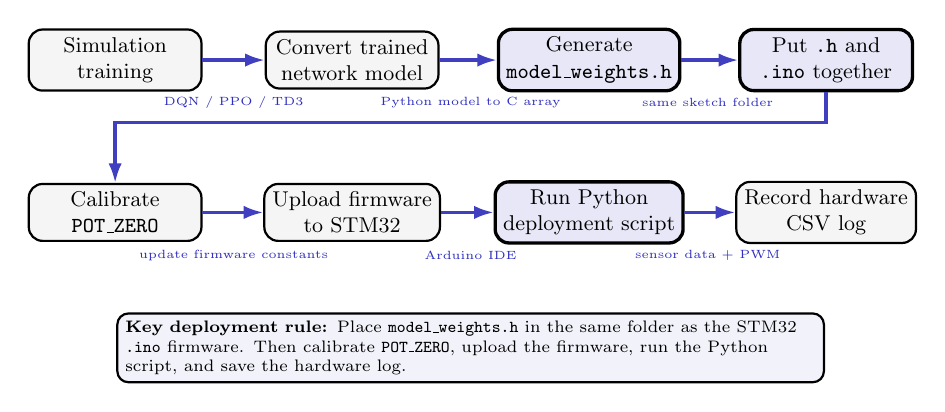
\begin{tikzpicture}[
    scale=0.86,
    transform shape,
    font=\small,
    >={Latex[length=2.5mm,width=1.7mm]},
    block/.style={
        draw,
        rounded corners=5pt,
        thick,
        align=center,
        minimum width=2.55cm,
        minimum height=0.82cm,
        fill=CodeGray
    },
    strong/.style={
        draw,
        rounded corners=5pt,
        very thick,
        align=center,
        minimum width=2.55cm,
        minimum height=0.82cm,
        fill=PKULightPurple!28
    },
    arrow/.style={
        ->,
        very thick,
        draw=PKUDarkPurple
    },
    note/.style={
        align=center,
        font=\tiny,
        text=PKUTextBlue
    }
]

% =========================
% Row 1: model preparation
% =========================
\node[block]  (train)  at (-5.25,1.55) {Simulation\\training};
\node[block]  (export) at (-1.75,1.55) {Convert trained\\network model};
\node[strong] (header) at (1.75,1.55) {Generate\\\texttt{model\_weights.h}};
\node[strong] (folder) at (5.25,1.55) {Put \texttt{.h} and\\\texttt{.ino} together};

\draw[arrow] (train.east) -- (export.west);
\draw[arrow] (export.east) -- (header.west);
\draw[arrow] (header.east) -- (folder.west);

\node[note] at (-3.50,0.92) {DQN / PPO / TD3};
\node[note] at (0.00,0.92) {Python model to C array};
\node[note] at (3.50,0.92) {same sketch folder};

% =========================
% Row 2: hardware deployment
% =========================
\node[block]  (calib)  at (-5.25,-0.70) {Calibrate\\\texttt{POT\_ZERO}};
\node[block]  (upload) at (-1.75,-0.70) {Upload firmware\\to STM32};
\node[strong] (runpy)  at (1.75,-0.70) {Run Python\\deployment script};
\node[block]  (log)    at (5.25,-0.70) {Record hardware\\CSV log};

\draw[arrow] (folder.south) -- ++(0,-0.45) -| (calib.north);
\draw[arrow] (calib.east) -- (upload.west);
\draw[arrow] (upload.east) -- (runpy.west);
\draw[arrow] (runpy.east) -- (log.west);

\node[note] at (-3.50,-1.33) {update firmware constants};
\node[note] at (0.00,-1.33) {Arduino IDE};
\node[note] at (3.50,-1.33) {sensor data + PWM};

% =========================
% Key message
% =========================
\node[
    draw,
    rounded corners=4pt,
    thick,
    align=left,
    fill=PKULightPurple!15,
    text width=10.2cm,
    font=\scriptsize
] at (0,-2.70) {
\textbf{Key deployment rule:}
Place \texttt{model\_weights.h} in the same folder as the STM32 \texttt{.ino} firmware.
Then calibrate \texttt{POT\_ZERO}, upload the firmware, run the Python script, and save the hardware log.
};

\end{tikzpicture}
\end{center}

\end{frame}


% ---------------------------------
\begin{frame}{Step 1: potentiometer zero calibration}
\begin{enumerate}
    \item Upload the raw sensor test firmware or use the deployment firmware serial output.
    \vspace{0.2cm}
    \item Hold the pendulum exactly near the upright position and keep it still.
    \vspace{0.2cm}
    \item Read the current potentiometer raw value \texttt{pot} from the serial monitor or log.
    \vspace{0.2cm}
    \item Set this value as \texttt{POT\_ZERO} in the firmware.
    \vspace{0.2cm}
    \item Re-upload the firmware after modifying \texttt{POT\_ZERO}.
\end{enumerate}


\end{frame}

% ---------------------------------
\begin{frame}[fragile]{Step 2: put model headers beside firmware}
\begin{lstlisting}[basicstyle=\ttfamily\scriptsize]
DQN sketch folder:
  deploy_dqn.ino
  model_weights.h

PPO sketch folder:
  deploy_ppo.ino
  ppo_model_weights.h
  dqn_model_weights.h

TD3 sketch folder:
  deploy_td3.ino
  td3_model_weights.h
\end{lstlisting}

\vspace{0.15cm}
\begin{alertblock}{Common mistake}
\small
If the header file is missing or has a mismatched format, Arduino IDE will fail during compilation. Always confirm that the header name matches the \texttt{\#include} line in the firmware.
\end{alertblock}
\end{frame}

% ---------------------------------
\begin{frame}{Step 3: upload firmware and close Serial Monitor}
\begin{enumerate}
    \item Open the corresponding \texttt{deploy\_*.ino} file in Arduino IDE.
    \vspace{0.25cm}
    \item Select the correct STM32 board and serial port.
    \vspace{0.25cm}
    \item Upload the firmware.
    \vspace{0.25cm}
    \item Close Arduino Serial Monitor after checking startup information.
    \vspace{0.25cm}
    \item Run the Python deployment script from a terminal.
\end{enumerate}

\vspace{0.15cm}
\begin{block}{Reason}
\small
Only one program can occupy the serial port. If Arduino Serial Monitor is still open, the Python logger cannot connect to STM32.
\end{block}
\end{frame}

% ---------------------------------
\begin{frame}[fragile]{Step 4: run the PC deployment logger}
\begin{lstlisting}[basicstyle=\ttfamily\scriptsize]
# DQN
python deploy_dqn.py

# PPO
python deploy_ppo.py

# TD3
python deploy_td3.py
\end{lstlisting}

\vspace{0.2cm}

The script will:
\begin{itemize}
    \item find or open the serial port;
    \item wait for the student to press Enter;
    \item send \texttt{GO} to STM32;
    \item record all \texttt{LOG} lines into a CSV file;
    \item send \texttt{S} when the experiment stops or falls.
\end{itemize}
\end{frame}

% ---------------------------------
% ---------------------------------
\begin{frame}{Deployment start modes}

\begin{center}
\begin{tabular}{c|c|c}
\hline
\textbf{Algorithm} & \textbf{Policy type} & \textbf{Student operation} \\
\hline
DQN &
swing-up + stabilization &
start from natural hanging-down state \\
\hline
TD3 &
swing-up + stabilization &
start from natural hanging-down state \\
\hline
PPO &
upright stabilization only &
hold near upright, press Enter, and release \\
\hline
\end{tabular}
\end{center}

\vspace{0.25cm}

\begin{alertblock}{Important start condition}
\small
The DQN and TD3 policies trained in simulation include the swing-up stage, so they can be tested from the natural hanging-down position.
The PPO policy used in this class is a balance-only policy, so students must gently hold the pendulum near the upright position, press Enter in the Python terminal, and release at the same time.
\end{alertblock}

\end{frame}


% ---------------------------------
\begin{frame}{Before pressing Enter}

Before sending the \texttt{GO} command from Python, check:

\begin{itemize}
    \item the correct model header has been compiled into the firmware;
    \vspace{0.18cm}

    \item \texttt{POT\_ZERO} has been updated for the current device;
    \vspace{0.18cm}

    \item motor power is connected only after wiring is checked;
    \vspace{0.18cm}

    \item the rotating arm has enough free space;
    \vspace{0.18cm}

    \item the emergency stop command is ready in the Python terminal.
\end{itemize}

\vspace{0.2cm}

\begin{alertblock}{Safety rule}
\small
Keep hands away from the rotating arm after pressing Enter.
If the pendulum falls or the motor behaves abnormally, stop the experiment immediately.
\end{alertblock}

\end{frame}


% ---------------------------------
\begin{frame}{What should be recorded?}

The Python logger should save one CSV file for each hardware test.

\vspace{0.18cm}

A useful deployment log should include:
\[
t,\quad
\theta,\quad
\alpha,\quad
\dot{\theta},\quad
\dot{\alpha},\quad
u,\quad
\text{mode}.
\]

\vspace{0.2cm}

Recommended additional fields:
\[
\text{pot\_raw},\quad
\text{enc},\quad
\text{action index},\quad
\text{done flag}.
\]

\vspace{0.2cm}

\begin{block}{Why log mode?}
\small
The mode field tells us whether the controller is in swing-up, stabilization, fallback, or safety-stop mode.
It is important for diagnosing failed deployment.
\end{block}

\end{frame}




% ---------------------------------
\begin{frame}{DQN deployment: what to check}

DQN uses a discrete action set.

\vspace{0.15cm}

During deployment, check:

\begin{itemize}
    \item whether the learned policy can swing the pendulum up from the natural hanging-down state;
    \vspace{0.18cm}

    \item whether the action sequence is reasonable rather than random-like switching;
    \vspace{0.18cm}

    \item whether the pendulum can enter and remain near the upright region;
    \vspace{0.18cm}

    \item whether PWM saturation appears too often.
\end{itemize}

\vspace{0.15cm}

\begin{alertblock}{Typical failure}
\small
If the real pendulum cannot swing up although simulation works, possible reasons include insufficient motor torque, wrong action scaling, friction mismatch, or wrong angle calibration.
\end{alertblock}

\end{frame}


% ---------------------------------
\begin{frame}{PPO deployment: what to check}

In this class, the PPO policy is used as an upright stabilization policy.

\vspace{0.15cm}

The correct start procedure is:

\begin{enumerate}
    \item hold the pendulum near the upright position;
    \vspace{0.16cm}

    \item run the Python deployment script;
    \vspace{0.16cm}

    \item press Enter to send \texttt{GO};
    \vspace{0.16cm}

    \item release the pendulum gently at the same time.
\end{enumerate}

\vspace{0.15cm}

\begin{block}{Evaluation}
\small
A good PPO deployment should keep \(\alpha\) close to zero after release and avoid high-frequency PWM oscillation.
\end{block}

\end{frame}


% ---------------------------------
\begin{frame}{TD3 deployment: what to check}

TD3 uses a continuous actor output.

\vspace{0.18cm}

During deployment, check:

\begin{itemize}
    \item whether the continuous action is correctly mapped to PWM;
    \vspace{0.18cm}

    \item whether the actor output is saturated too frequently;
    \vspace{0.18cm}

    \item whether the pendulum can swing up and stabilize in the real system;
    \vspace{0.18cm}

    \item whether the real response is smoother or more unstable than DQN.
\end{itemize}

\vspace{0.15cm}

\begin{alertblock}{Important}
\small
A continuous actor may generate smoother commands in simulation, but real motor dead zone and friction can strongly change its behavior.
\end{alertblock}

\end{frame}


% ---------------------------------
\begin{frame}{Simulation-to-hardware comparison}

For each algorithm, compare simulation and hardware results.

\vspace{0.2cm}

\begin{center}
\begin{tabular}{c|c|c}
\hline
\textbf{Item} & \textbf{Simulation} & \textbf{Hardware} \\
\hline
Initial condition & controlled setting & real manual / natural start \\
\hline
Sensor signal & clean or simulated noise & real noise and drift \\
\hline
Motor response & ideal mapping & dead zone and saturation \\
\hline
Time step & fixed simulation step & real sampling jitter possible \\
\hline
Control curve & expected rollout & measured CSV log \\
\hline
\end{tabular}
\end{center}

\vspace{0.15cm}

\begin{block}{Goal}
\small
The goal is not only to show whether the controller works, but also to explain why simulation and hardware differ.
\end{block}

\end{frame}





% ---------------------------------
\begin{frame}{Common sim-to-real mismatch sources}

\begin{itemize}
    \item \textbf{Angle calibration error:}
    wrong \texttt{POT\_ZERO} shifts the definition of \(\alpha=0\).
    \vspace{0.18cm}

    \item \textbf{Motor dead zone:}
    small PWM commands may not move the motor.
    \vspace{0.18cm}

    \item \textbf{Friction and backlash:}
    real mechanical resistance is not perfectly modeled.
    \vspace{0.18cm}

    \item \textbf{Sensor noise:}
    angle difference can amplify noise in velocity estimation.
    \vspace{0.18cm}

    \item \textbf{Delay and timing jitter:}
    serial communication and real-time loop timing may differ from simulation.
\end{itemize}

\end{frame}


% ---------------------------------
\begin{frame}{How to diagnose a failed deployment}

\begin{center}
\begin{tabular}{c|p{0.60\textwidth}}
\hline
\textbf{Symptom} & \textbf{Possible reason} \\
\hline
Motor does not move & motor power off, wrong PWM mapping, motor dead zone \\
\hline
Moves in wrong direction & sign error in angle, encoder, or PWM command \\
\hline
Falls immediately near upright & wrong \texttt{POT\_ZERO}, policy not trained for this state region \\
\hline
Strong oscillation & excessive gain, noisy velocity estimate, delay, unstable policy \\
\hline
Works in simulation only & model mismatch, friction, saturation, unmodeled delay \\
\hline
\end{tabular}
\end{center}

\vspace{0.2cm}


Do not change many parameters at the same time.
Change one factor, record the result, and compare the log.


\end{frame}


% ---------------------------------
\begin{frame}{Report requirements}

Each group should include:

\begin{itemize}
    \item deployment procedure for DQN, PPO, and TD3;
    \vspace{0.12cm}

    \item model header file name and firmware file name;
    \vspace{0.12cm}

    \item calibrated \texttt{POT\_ZERO} value;
    \vspace{0.12cm}

    \item simulation rollout plots for the deployed models;
    \vspace{0.12cm}

    \item hardware deployment plots and CSV logs;
    \vspace{0.12cm}

    \item comparison of DQN, PPO, and TD3 real-system performance;
    \vspace{0.12cm}

    \item sim-to-real mismatch analysis.
\end{itemize}

\vspace{0.15cm}

\begin{block}{Main focus}
\small
The report should connect the simulation training result with the real hardware behavior.
\end{block}

\end{frame}

% ---------------------------------
\begin{frame}{Suggested quantitative metrics}

For DQN and TD3, record the swing-up performance:
\[
T_{\mathrm{swing}},
\qquad
T_{\mathrm{upright}},
\qquad
N_{\mathrm{fall}}.
\]

\vspace{0.15cm}

For all deployed algorithms, evaluate the stabilization stage:
\[
\mathrm{mean}(|\alpha|),
\qquad
\mathrm{std}(\alpha),
\qquad
\mathrm{mean}(|\theta|),
\qquad
\mathrm{std}(\theta).
\]

\vspace{0.15cm}

Also report PWM usage:
\[
\mathrm{mean}(|u|),
\qquad
\max(|u|),
\qquad
\text{saturation ratio}.
\]

\vspace{0.12cm}


DQN and TD3 include swing-up, so \(T_{\mathrm{swing}}\) should be recorded.
PPO is used as an upright stabilization policy in this class, so only the stabilization-stage accuracy and PWM usage are evaluated.


\end{frame}


% ---------------------------------
\begin{frame}{Required plots for deployment analysis}

For each algorithm, plot the following time histories:
\[
\theta(t),\qquad
\alpha(t),
\qquad
\dot{\theta}(t),
\qquad
\dot{\alpha}(t).
\]

\vspace{0.18cm}

Also plot the PWM command:
\[
u(t).
\]

\vspace{0.18cm}

For PWM statistics, include at least one summary figure:
\[
\text{PWM histogram}
\qquad \text{or} \qquad
\text{bar chart of } \mathrm{mean}(|u|),\ \max(|u|),\ \text{saturation ratio}.
\]

\vspace{0.15cm}

\begin{alertblock}{Comparison requirement}
\small
Use the same angle convention, time unit, and PWM scale when comparing DQN, PPO, and TD3.
For DQN and TD3, mark the swing-up stage and the stabilization stage on the plot if possible.
\end{alertblock}

\end{frame}
% ---------------------------------



% ---------------------------------
\begin{frame}{Suggested report structure}

\begin{enumerate}
    \item Brief description of deployed models and firmware.
    \vspace{0.12cm}

    \item Sensor calibration and hardware start conditions.
    \vspace{0.12cm}

    \item DQN deployment result and analysis.
    \vspace{0.12cm}

    \item PPO deployment result and analysis.
    \vspace{0.12cm}

    \item TD3 deployment result and analysis.
    \vspace{0.12cm}

    \item Cross-algorithm comparison.
    \vspace{0.12cm}

    \item Sim-to-real mismatch discussion.
    \vspace{0.12cm}

    \item Possible improvements for the next class.
\end{enumerate}

\end{frame}


% ---------------------------------
\begin{frame}{Summary of Class 11}

\begin{itemize}
    \item We moved from simulation-trained policies to real STM32 deployment.
    \vspace{0.2cm}

    \item We learned the workflow:
    model weights, firmware, sensor calibration, Python logger, and hardware CSV logs.
    \vspace{0.2cm}

    \item DQN and TD3 are tested as swing-up plus stabilization policies.
    \vspace{0.2cm}

    \item PPO is tested as a balance-only policy near the upright region.
    \vspace{0.2cm}

    \item The most important analysis is the difference between simulation behavior and real hardware behavior.
\end{itemize}

\vspace{0.2cm}

\begin{alertblock}{Take-home message}
\small
Successful AI-enabled control requires not only training a policy, but also deploying it safely, recording real data, and explaining the sim-to-real gap.
\end{alertblock}

\end{frame}


\end{document}
